%
% multipol.tex
%
% (c) 2017 Prof Dr Andreas Müller, Hochschule Rapperswil
%
\chapter{Multipolentwicklung
\label{skript:chapter:multipol}}
\lhead{Multipole und CMB}
\rhead{}
Beobachtet man ein kleines Objekt aus einiger Distanz sind viele
Details nicht mehr erkennbar.
Dieses Ph"anomen muss auch einen mathematischen Ausdruck haben.

Eine Masseverteilung wird ein Gravitationsfeld haben, welches aus
grosser Distanz kaum unterscheidbar sein wird vom Gravitationsfeld
eines einzelnen Masspunktes.
Eine Ladungsverteilung erzeugt ein elektrisches Feld, welches in
grosser Entfernung mit $\frac1r$ abfällt.
Ist die Gesamtladung $0$, bedeutet das aber nicht, dass das
Feld vollständig verschwindet, es bleibt ein Restfeld, welches
allerdings mit $\frac1{r^2}$ abfällt.
In all diesen Fällen haben wir es mit einer Funktion $f(x,y,z)$ zu tun,
die für vergleichsweise kleine Werte der Koordinaten $x$, $y$ und $z$
nur schwer im Detail verstehen können.
Uns interessiert aber vor allem das Verhalten für grosse Werte der
Koordinaten, also weit von den unverständlichen Details entfernt.

Neben dem Abfall der Funktionswerte mit der Entfernung ist auch
die Verteilung der Funktionswerte in verschiedenen Richtungen wesentlich.
Wir erwarten also, dass wir jede beliebige Funktion in Terme der Form
$
f(r) g(\vartheta,\varphi)
$
zu zerlegen, worin $f(r)$ nur von der Entfernung und $g(\vartheta,\varphi)$
nur von geographischer Länge und Breite der Richtung abhängt.
Dabei ist immer noch möglich, das verschieden schnell abfallende
Terme verschiedene Richtungsverteilungen haben.

Wir werden im nächsten Kapitel eine Familie von Funktionen
von $\vartheta$ und $\varphi$ entwickeln, die Kugelfunktionen,
mit welchen wir die Richtungsabhängigkeit untersuchen können.
Zusammen mit verschiedenen Funktionen, die die Entfernungsabhängigkeit
beschreiben, erhalten wir so ein Instrumentarium zur Analyse von
beliebigen Funktionen.

In diesem Kapitel beginnen wir damit, den Spezialfall des Potentials
etwas genauer zu studieren.
Dabei zeigen sich bereits einige Eigenschaften, aus denen sich
später die Theorie der Kugelfunktionen ganz natürlich ergibt.

%
% m-1dim.tex -- ein eindimensionales Beispiel
%
% (c) 2017 Prof Dr Andreas Müller, Hochschule Rapperswil
%
\section{Ein eindimensionales Beispiel%
\label{skript:multipol:1dimbeispiel}}
\rhead{Ein eindimensionales Beispiel}
In diesem Abschnitt betrachten wir eine Funktion, die nur von einer
Variablen $x$ abhängt.
Es interessiert uns in erster Linie ihr Verhalten 
für $x\to\pm\infty$.
Wir führen dazu eine Methode vor, die sich leicht auf die dreidimensionale
Situation ausweiten lässt.

\subsection{Monopol und Dipol}
Das Potential einer Ladung $e$ fällt mit der Entfernung $r$ nach dem
Coulomb-Gesetz
\index{Coulomb-Gesetz}%
\[
f(r)=\frac1{4\pi\varepsilon_0}\frac{q}r
\]
ab.
Platziert man die Ladung $q$ im Punkt $a$ eines eindimensionalen
Koordinatensystems, dann ist das Potential in Abhängigkeit von $x$
\begin{equation}
f_1(x) = \frac{q}{4\pi\varepsilon_0} \frac1{|x-a|}.
\label{skript:multipol:1monopol}
\end{equation}
Für $x>a$ kann man \eqref{skript:multipol:1monopol} schreiben als
\begin{equation}
f_1(x)
=
\frac{q}{4\pi\varepsilon_0} \frac1{x-a}
=
\frac{q}{4\pi\varepsilon_0} \frac1x\frac1{1-\displaystyle\frac{a\mathstrut}{x}}.
\label{skript:multipol:1abfall}
\end{equation}
Im letzten Faktor kann man ablesen, dass der Summand $a/x$ im Nenner
auf der rechten Seite für grosse $x$ unbedeutend wird, so dass $f(x)$
immer noch wie $1/x$ abfällt, unabhängig davon, wo die Ladung platziert
wird.

\begin{figure}
\centering
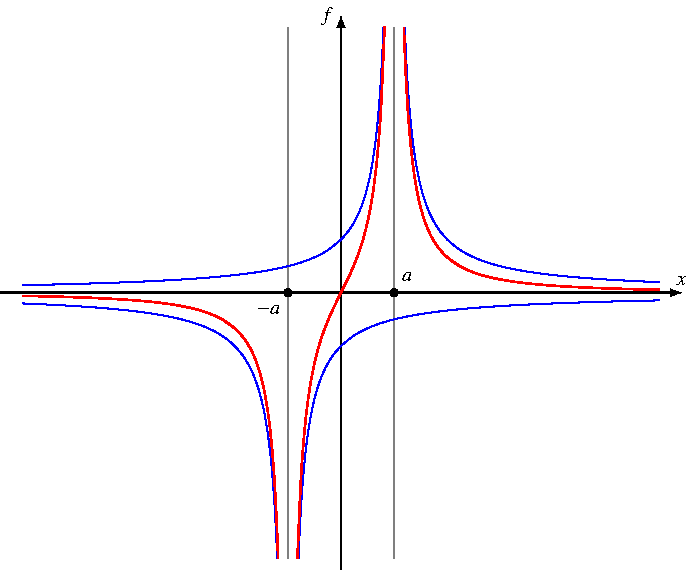
\includegraphics{chapters/tikz/dipol1.pdf}
\caption{Potential
\eqref{skript:multipol:1dipol}
des eindimensionalen Dipols
\label{skript:multipol:figure:1dim}}
\end{figure}

Zwei entgegengesetzte Punktladungen an den Stellen $x=\pm a$ haben also
das Potential
\begin{equation}
f_2(x)
=
\frac1{4\pi\varepsilon_0}\frac{q}{|x+a|}
-
\frac1{4\pi\varepsilon_0}\frac{q}{|x-a|}
=
\frac{q}{4\pi\varepsilon_0}\biggl( \frac1{|x+a|} - \frac1{|x-a|} \biggr).
\label{skript:multipol:1dipol}
\end{equation}
(Abbildung~\ref{skript:multipol:figure:1dim}).
Wir sind nur an den Funktionswerten interessiert für $x$-Werte, die
wesentlich grösser sind als $a$, als in grosser Entfernung von
den Ladungen.
Wir interessieren uns also für $x$-Werte so, dass $x/a$ sehr gross ist,
oder umgekehrt, dass $a/x$ sehr klein ist.

Wenn man in Gleichung \eqref{skript:multipol:1dipol} das Vorzeichen
von $x$ kehrt, dann ändert das Vorzeichen von $f$, also $f_2(-x)=-f_2(x)$,
$f$ ist eine ungerade Funktion.
Es reicht daher, die Funktion $f_2(x)$ für $x\gg a$ zu untersuchen,
für Werte $x\ll -a$ verwendet man $f_2(x)=-f_2(-x)$.

Verwenden wir die Gleichung \eqref{skript:multipol:1abfall} in $f_2(x)$,
erhalten wir
\begin{align}
f_2(x)
&=
\frac{q}{4\pi\varepsilon_0}\biggl(\frac1{x+a}-\frac1{x-a}\biggr)
=
\frac{q}{4\pi\varepsilon_0}\cdot\frac1x\cdot\biggl(
\frac1{1+\frac{a\mathstrut}{x}}
-
\frac1{1-\frac{a\mathstrut}{x}}
\biggr)
=
\frac{q}{4\pi\varepsilon_0}\cdot\frac1x\cdot
\frac{\bigl(1-\frac{a}{x}\bigr)-\bigl(1+\frac{a}{x}\bigr)}{1-\frac{a^2}{x^2}}
\notag
\\
&=
\frac{q}{4\pi\varepsilon_0}\cdot\frac1x\cdot
\biggl(-\frac{2a}{x}\biggr)
\cdot
\frac1{1-\frac{a^2}{x^2}}
=
-\frac{qa}{2\pi\varepsilon_0}\cdot\frac1{x^2}\cdot\frac{1}{1-\frac{a^2}{x^2}}.
\label{skript:multipol:2abfall}
\end{align}
Der Term $a^2/x^2$ im Nenner des letzten Faktors ist für grosse Werte von
$x$ wieder unbedeutend.
Der dominierende Term für das Verhalten für grosse $x$ ist daher der
Faktor $1/x^2$.

Ein weiterer interessanter Aspekt der Formel~\eqref{skript:multipol:2abfall}
ist, dass nur noch die Kombination $qa$ von Ladung und Abstand der Ladungen
vorkommt.
Das Fernfeld für grosse Werte von $x$ ändert also nicht, wenn wir $a$
kleiner machen, aber gleichzeitig $q$ vergrössern, so dass das Produkt
$qa$ konstant bleibt.
Man nennt $d=2qa$ das {\em Dipolmoment} der beiden Ladungen.
\index{Dipolmoment}%
Der Dipol mit Dipolmoment $d$ hat daher für grosse $x$ das Potential
\[
f_2(x)
=
-\frac{d}{4\pi\varepsilon_0}\cdot \frac1{x^2}\cdot \frac1{1-\frac{a^2}{x^2}}
\simeq
-\frac{d}{4\pi\varepsilon_0}\cdot \frac1{x^2}.
\]

Aus diesen Beispielen können wir die Vermutung ableiten, dass weitere
Terme die Form
\[
-\frac{b}{4\pi\varepsilon_0}\cdot\frac1{x^k}
\]
haben müssen, wobei $b$ die Dimension einer Ladung mal die $(k-1)$-te
Potenz einer Distanz sein muss.

\subsection{Stetige Ladungsverteilung%
\label{skript:multipol:section:stetigeladungsverteilung}}
Betrachten wir jetzt statt zweier Ladungen eine beliebige 
Ladungsverteilung $\varrho(x)$, die aber ausserhalb des Intervalls
$[-a,a]$ verschwindet, also $\varrho(x)=0$ für $|x|>a$.
Stellen wir uns die Ladungsverteilung als eine Überlagerung einzelner
Ladungen an Positionen $y\in[-a,a]$ vor, dann k"onnen wir das
Potential des Fernfeldes sofort aus~\eqref{skript:multipol:2abfall}
ableiten:
\[
f(x)
\simeq
\frac{1}{4\pi\varepsilon_0}
\underbrace{\int_{-a}^a \varrho(y)\,dy }_{\displaystyle =q}
\frac1x
+
\frac{1}{4\pi\varepsilon_0}
\underbrace{\int_{-a}^a \varrho(y)y \,dy}_{\displaystyle =d}
\frac1{x^2}
+
\dots
=
\frac{1}{4\pi\varepsilon_0}
\sum_{k=0}^\infty
\frac1{x^{k+1}} 
\int_{-a}^a\varrho(y)y^k\,dy
\]
Der erste Term ist das Potential einer Punktladung $q$ im Ursprung, der
zweite das Dipolpotential eines Dipols mit Dipolmoment $d$.
Wir nennen den ersten Term auch den {\em Monopolterm}.
\index{Monopol}%

Die Integrale 
\[
b_k=\int_{-a}^a \varrho(y)\,y^k\,dy
\]
heissen die {\em $k$-ten Momente} der Verteilung $\varrho$.
\index{Moment einer Funktion}%
Die $k$-ten Momente bestimmen also die Darstellung des Fernfeldes
einer Ladungsverteilung vollständig durch die Formel
\[
f(x)
\simeq
\frac1{4\pi\varepsilon_0}\sum_{k=0}^\infty b_k\frac{1}{x^{k+1}}.
\]
Wir behaupten nicht, dass die Summe auf der rechten Seite mit dem Potential
der Ladungsverteilung übereinstimmen.
Vielmehr ist die Summe eine Zerlegung des Feldes
nach ``Abfalls-Geschwindigkeit'' in grosser Entfernung,
ganz ähnlich wie die Fourier-Koeffizienten
\[
a_k=\frac1{2\pi}\int_{-\pi}^\pi f(x)\cos kx\,dx
\qquad\text{und}\qquad
b_k=\frac1{2\pi}\int_{-\pi}^\pi f(x)\sin kx\,dx
\]
einer im Intervall $[-\pi,\pi]$ definierten Funktion $f(x)$
eine Analyse nach Frequenzen bilden.
Die Fourierreihe
\[
\frac{a_0}2+\sum_{k=1}^\infty (a_k\cos kx+b_k\sin kx)
\]
ist eine periodische Funktion auf der ganzen reellen Achse, die
im Intervall $[-\pi,\pi]$ mit der ursprünglichen Funktion übereinstimmt.
Die Summe stimmt also mit der ursprünglichen Funktion nicht direkt
überein.

\subsection{Geometrische Reihe%
\label{skript:multipol:section:geometrischereihe}}
Bei der Analyse sowohl einer um $a$ verschobenen Einzelladung sowie auch
des Dipols aus zwei Ladungen bei $\pm a$ haben wir am Schluss Terme der
Form
\[
\frac1{1-\displaystyle\frac{a}{x}}
\qquad\text{bzw.}\qquad
\frac1{1-\displaystyle\frac{a^2}{x^2}}
\]
vernachlässigt.
Wir suchen nach einer Möglichkeit, diese Terme exakt zu berücksichtigen,
und trotzdem nur eine einfache Potenzreihe zu bekommen.

In der Analysis lernt man, die Summe der {\em geometrische Reihe}
\index{geometrische Reihe}
\index{Reihe, geometrische}
\[
s=a+aq+aq^2+\dots + aq^n
\]
zu berechnen.
Dazu bildet man $qs - s$ und findet
\begin{align*}
qs-s
=
s(q-1)
&=
q(a+aq+aq^2+\dots + aq^n)-(a+aq+aq^2+\dots + aq^n)
\\
&=
a(q+q^2+q^3\dots+q^{n+1}-1-q-q^2-\dots-q^n)
=
a(q^{n+1}-1).
\end{align*}
Daraus schliesst man
\[
s=a\frac{q^{n+1}-1}{q-1}.
\]
Wenn $|q|<1$ ist, dann kann man die Summe für beliebig grosse $n$ bilden,
und bekommt im Grenzwert $n\to\infty$
\begin{equation}
\sum_{k=0}^\infty aq^k = a\frac{1}{1-q}.
\label{skript:multipol:geom}
\end{equation}
Wir können diese Formel verwenden, um die bisher vernachlässigten Terme
exakt wiederzugeben:
\begin{align*}
\frac{1}{1-\displaystyle\frac{a}{x}}
&=
1+\frac{a}{x}+\frac{a^2}{x^2}+\dots
=
\sum_{k=0}^\infty \frac{a^k}{x^k},
\\
\frac{1}{1-\displaystyle\frac{a^2}{x^2}}
&=
1+\frac{a^2}{x^2}+\frac{a^4}{x^4}+\dots
=
\sum_{k=0}^\infty \frac{a^{2k}}{x^{2k}},
\\
\frac{1}{1+\displaystyle\frac{a^2}{x^2}}
&=
1-\frac{a^2}{x^2}+\frac{a^4}{x^4}-\dots
=
\sum_{k=0}^\infty (-1)^k\frac{a^{2k}}{x^{2k}}.
\end{align*}
Die letzte Formel erhält man, indem man in \eqref{skript:multipol:geom}
$q$ durch $-q$ ersetzt und dann $q=a^2/x^2$ einsetzt.

Wir wenden dies jetzt wieder auf eine Ladungsverteilung
$\varrho(y)$ im Intervall $[-a,a]$ an.
Das Potential einer Einheitsladung an der Stelle $y$ ist
\[
f_y(x)
=
\frac1{4\pi\varepsilon_0}\cdot \frac{1}{x}\cdot\frac{1}{1-\displaystyle\frac{x}{y}}
=
\frac1{4\pi\varepsilon_0}\cdot \frac{1}{x}
\sum_{k=0}^\infty \frac{y^k}{x^k}
=
\frac1{4\pi\varepsilon_0}
\sum_{k=0}^\infty \frac{y^k}{x^{k+1}}.
\]
Durch Überlagerung mit Hilfe der Ladungsverteilung $\varrho(y)$ 
erhalten wir die exakte Formel für das Potential der Ladungsverteilung
\begin{equation}
f(x)
=
\int_{-a}^af_y(x)\,dy
=
\frac{1}{4\pi\varepsilon_0}
\sum_{k=0}^\infty
\frac{1}{x^{k+1}}
\underbrace{\int_{-a}^a\varrho(y)\,y^k\,dy}_{\displaystyle =b_k}
\cdot
=
\frac{1}{4\pi\varepsilon_0}
\sum_{k=0}^\infty b_k
\frac{1}{x^{k+1}},
\label{skript:multipol:reiheexakte}
\end{equation}
wobei die $b_k$ wieder die $k$-ten Momente der Ladungsverteilung
$\varrho(y)$ sind.

Es stellt sich also heraus, dass die in
Abschnitt~\ref{skript:multipol:section:stetigeladungsverteilung}
erratene Entwicklung sogar eine exakte Darstellung ist.
Bricht man die Reihe~\eqref{skript:multipol:reiheexakte} nach zwei
Termen ab, erhält man die Monopol- und Dipol-Komponenten des
Fernfeldes.
Alle späteren Terme der Reihe beschreiben die feineren Strukturen
der Ladungsverteilung und fallen so rasch mit der Entfernung ab,
dass sie für grosse Entfernungen vernachlässigt werde können.

Bei der Diskussion des Dipolmoments haben wir festgestellt, dass das
Fernfeld nur von der Grösse $d=2aq$ abhängt.
Verkleinert man den Abstand $a$ und vergrössert man gleichzeitig $q$,
so dass $d$ gleich gross bleibt, dann ändert sich das Fernfeld nicht.
Die Reihe~\eqref{skript:multipol:reiheexakte} verallgemeinert diese
Aussage auf eine beliebige Ladungsverteilung.
Ändern wir die Ladungsverteilung, achten aber darauf, dass die
$k$-ten Momente gleich bleiben, dann ändert sich das ausserhalb der
Ladungsverteilung messbare Potential nicht.
Die $k$-ten Momente beschreiben das ausserhalb der Ladungsverteilung
messbare Potential vollständig.

\subsection{Taylor-Reihe und Laurent-Reihe}
Im vorangegangenen Abschnitt haben wir gesehen, dass für grosse Werte von
$x$ die zur Diskussion stehende Funktion im Wesentlichen als Reihe
der inverse Potenzen $1/x^k$ beschrieben werden kann, also
\[
f(x)=\sum_{k=0}^\infty b_k\frac1{x^{k+1}}.
\]
Schreiben wir $z=1/x$, dann wird daraus eine gewöhnliche Potenzreihe
\[
\tilde f(z)=\sum_{k=0}^\infty b_k z^{k+1}.
\]
Wenn die Funktion $z\mapsto \tilde f(z)$ differenzierbar ist, dann
können die Koeffizienten $b_k$ aus den Ableitungen der Funktion
$\tilde f$ gefunden
\begin{equation}
b_k=\frac{\tilde f^{(k)}(0)}{k!}
\qquad\Rightarrow\qquad
\tilde f(z)
=
\sum_{k=0}^\infty \frac{\tilde f^{(k)}(0)}{k!}z^k.
\end{equation}
Wir können dies betrachten als die Taylorreihe der Funktion $f$ um
den Punkt $\infty$.
\index{Taylor-Reihe}

Man nennt eine Reihe der Form
\[
\sum_{k=-\infty}^{\infty} b_k(z-a)^k
\]
eine {\em Laurent-Reihe} im Punkt $a$.
\index{Laurent-Reihe}
Offensichtlich ist der Funktionswert in $z=a$ nicht definiert und
oft wird die Reihe auch in einer Umgebung von $a$ nicht konvergieren.
Sie ist aber hervorragend dazu geeignet, das Verhalten einer Funktion
zu analysieren, die im Punkt $a$ eine Singularität aufweist.
Besonders nützlich ist sie dann, wenn $z$ komplex ist, denn man
kann zeigen, dass jede komplex differenzierbare Funktion mit einer
Singularität im Punkt $a$ in einer Umgebung von $a$ als Laurent-Reihe
dargestellt werden kann \cite{skript:mathsemdgl}.

Wenn wir also in der Lage sind, das eindimensionale Beispiel auf höhere
Dimensionen zu verallgemeinern, dann haben wir auch eine Verallgemeinerung
der Idee einer Taylorreihe um den Punkt $\infty$ auf höhere Dimensionen
gefunden.









%
% m-multipole.tex
%
% (c) 2017 Prof Dr Andreas Müller, Hochschule Rapperswil
%
\section{Multipolentwicklung}
\rhead{Multipolentwicklung}
In Abschnitt~\ref{skript:multipol:1dimbeispiel} haben wir ein
eindimensionales Beispiel untersucht, und mussten nach dem Potential
eines Dipols mit Vermutungen operieren, wie die weiteren Terme aussehen
müssten.
In diesem Abschnitt arbeiten wir in drei Dimensionen, und sind daher
in der Lage, kompliziertere Konfigurationen von Ladungen zu
konstruieren, und damit auch die späteren Terme der Entwicklung
genauer zu untersuchen.


\subsection{Dipol}
\begin{figure}
\centering
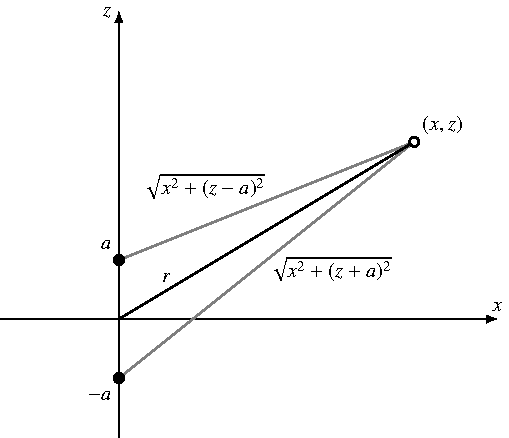
\includegraphics{chapters/tikz/dipol2.pdf}
\caption{Berechnung des Dipolpotentials 
\eqref{skript:multipol:dipol} in der $x$-$z$-Ebene
\label{skript:multipol:figure:dipol}}
\end{figure}
Wir betrachten das Feld eines Paares von entgegengesetzen Ladungen
in den Punkten $(0,0,a)$ und $(0,0,-a)$
(Abbildung~\ref{skript:multipol:figure:dipol}).
Der Einfachheit halber führen wir die Rechnung zunächst nur
in der $x$-$z$-Ebene durchführen und erst später mit Hilfe einer
vektoriellen Schreibweise auf drei Dimensionen erweitern.

Entlang der $z$-Achse kennen wir das Potential bereits aus
dem vorangegangenen Abschnitt.
Entlang der $x$-Achse verschwindet das Potential, denn die Punkte
auf der $x$-Achse sind von den beiden Ladungn gleich weit entfernt,
haben als entgegengesetzt gleiches Potential bezüglich beiden Ladungen
und damit totales Potential 0.

Wir betrachten jetzt das Potential im Punkt $(x,z)$, es ist
\begin{equation}
f(x,z)
=
\frac{q}{4\pi\varepsilon_0}
\biggl(
\frac{1}{\sqrt{x^2 + (z-a)^2}}
-
\frac{1}{\sqrt{x^2 + (z+a)^2}}
\biggr)
\label{skript:multipol:dipol}
\end{equation}
Offenbar müssen wir die Nenner besser verstehen, um diese Summe 
umformen zu können.
Speziell müssen wir die Abhängigkeit von der Entfernung
$r=\sqrt{x^2+z^2}$ vom Nullpunkt
und die Richtungsabhängigkeit voneinander trennen.
Dazu betrachten wir nur einen einzelnen Term
\[
\frac{1}{\sqrt{x^2+(z\pm a)^2}}
=
\frac{1}{\sqrt{x^2+z^2\pm 2az+a^2}}
=
\frac{1}{\sqrt{x^2+z^2}} \cdot \frac{1}{\sqrt{1+\frac{\pm 2az+a^2}{x^2+z^2}}}
=
\frac{1}{r} \cdot \frac{1}{\sqrt{1+\frac{\pm 2az+a^2}{r^2}}}
\]
Für grosse Werte von $r$ verschwindet der zweite Term in der Wurzel,
in erster Näherung verhält sich die Funktion daher wie $1/r$.
In den zwei Termen von \eqref{skript:multipol:dipol} hebt sich dieses
Verhalten jedoch weg, um die Funktion $f(x,z)$ zu verstehen, ist es
daher nötig, die Abweichungen von $1/r$ genauer zu verstehen.

Offenbar müssen wir Terme der Form
\begin{equation}
\frac{1}{\sqrt{1+t}}
=
(1+t)^{-\frac12}
\label{skript:multipol:wurzel}
\end{equation}
ausrechnen können, wobei wir später $t=(\pm2az+a^2)/r^2$ setzen wollen.

\subsubsection{Binomialreihe}
Die Taylor-Reihe der Funktion \eqref{skript:multipol:wurzel}
kann für eine allgemeinere für die Funktionen
\begin{equation}
g(t)=(1+t)^\alpha
\end{equation}
mit beliebigem Exponenten bestimmt werden.

Dazu müssen die Ableitungen der Funktion $g(t)$ bestimmt werden
\begin{align*}
g'(t)
&=
\alpha(1+t)^{\alpha-1}
&
g'(0)&=\alpha
\\
g''(t)
&=
\alpha(\alpha-1)(1+t)^{\alpha-2}
&
g''(0)&=\alpha(\alpha-1)
\\
&\;\vdots
\\
g^{(n)}(t)
&=
\alpha(\alpha-1)(\alpha-2)\dots(\alpha-n+1) (1+t)^{\alpha -n}
&
g^{(n)}(0)&=\alpha(\alpha-1)(\alpha-2)\dots(\alpha -n +1)
\end{align*}
Der Term zur Potenz $n$ in der Taylor-Reihe von $g(t)$ ist
\[
\frac{\alpha(\alpha-1)(\alpha-2)\dots(\alpha-n+1)}{n!} t^n
\]
Wäre $\alpha$ eine ganze Zahl, dann sähe der Bruch
genau so aus wie der Binomialkoeffizient $\binom{\alpha}{k}$.
In Erweiterung der üblichen Definition des Binomialkoeffizienten
schreibt man auch für nicht ganzzahlige $\alpha$
\[
\binom{\alpha}{n}
=
\frac{\alpha(\alpha-1)(\alpha-2)\dots(\alpha-n+1)}{n!}.
\]
Mit dieser Schreibweise bekommen wir die Taylorreihe
\[
(1+t)^\alpha=\sum_{k=1}^\infty \binom{\alpha}{k} t^k
\]
für die Funktion $(1+t)^\alpha$.
Sie heisst die {\em Binomialreihe} und ist konvergent für $|t|<1$.
\index{Binomialreihe}

\subsubsection{Der Fall $\alpha=-\frac12$}
Wir betrachten die Binomialreihe für den Fall $\alpha=-\frac12$.
Der Term zur Potenz $n$ ist
\begin{equation}
\frac{
\bigl(-\frac12\bigr)
\bigl(-\frac32\bigr)
\bigl(-\frac52\bigr)
\cdots
\bigl(-\frac{2n+1}2\bigr)}{n!} t^n
=
(-1)^n \frac{1\cdot 3\cdot 5 \cdots (2n + 1)}{2^n\cdot 1\cdot 2\cdot 3\cdots n}
=
(-1)^n \frac{1\cdot 3\cdot 5 \cdots (2n+1)}{2\cdot 4\cdot 6\cdots (2n)}
\label{skript:multipol:koeffizienten}
\end{equation}
Die zugehörige Potenzreihe ist daher
\[
\frac1{\sqrt{1+t}}
=
1-\frac12t+\frac3{8}t^2-\frac{15}{48}t^3+\frac{105}{354}t^4-\dots
\]
%deren Koeffizienten man auch faktorisieren und damit etwas
%Für 
%\[
%\frac1{\sqrt{1+t}}
%=
%1-\frac12 t
%+ \frac12\frac32\frac12 t^2
%- \frac 12\frac32\frac 52\frac1{3!} t^3
%+ \frac 12\frac32\frac 52\frac72\frac1{4!} t^4
%- \frac 12\frac32\frac 52\frac72\frac92\frac1{5!} t^4
%+\dots
%\]

Wir verwenden die binomische Reihe jetzt, um das Dipolpotential
zu berechnen.
Setzen wir 
\[
t=\frac{\pm 2az+a^2}{r^2}
\]
in der binomischen Reihe, erhalten wir
\[
\frac{1}{\sqrt{1+\frac{\pm 2az+a^2}{r^2}}}
=
1-\frac12\frac{\pm 2az+a^2}{r^2}
+
\frac38 \biggl(\frac{\pm 2az+a^2}{r^2}\biggr)^2+\dots
\]
und für das Dipolpotential $f(x,z)$ gemäss \eqref{skript:multipol:wurzel}
\begin{align*}
f(x,z)
&=
\frac{q}{4\pi\varepsilon_0 r}
\biggl(
1-\frac12\frac{-2az+a^2}{r^2} + \frac38 \biggl(\frac{-2az+a^2}{r^2}\biggr)^2+\dots
\biggr)
\\
&\qquad
-
\frac{q}{4\pi\varepsilon_0 r}
\biggl(
1-\frac12\frac{2az+a^2}{r^2} + \frac38 \biggl(\frac{2az+a^2}{r^2}\biggr)^2+\dots
\biggr)
\\
&=
-\frac{2aq}{4\pi\varepsilon_0r^3}z + \dots
\end{align*}
Wenn die beiden Ladungen näher zusammen rücken, wenn also $a\to 0$,
dann verschwindet das Potential.
Wenn wir das Potential weiterhin sehen wollen, müssen wir den Betrag
der Ladungen entsprechend vergrössern.
Wenn wir $a$ gegen $0$ gehen lassen, lassen wir gleichzeit die Ladung
$q$ grösser werden, so dass das Produkt $d=2qa$ gleich bleibt.
Mit dieser Konvention wird das Dipolpotential
\begin{equation}
f(x,z) = -\frac{d}{4\pi\varepsilon_0 r^2}\frac{z}{r}+\dots
\label{skript:multipol:dipolpotential}
\end{equation}
Darin haben wir statt $z$ den Bruch $z/r$ abgespalten, da dieser
eintlang eines vom Nullpunkt ausgehenden Strahls vom Zentrum jeweils
konstant ist.
Wir haben daher das Potential in Faktoren aufgeteilt, die verschiedene
geometrische Bedeutung haben.
Der Faktor $1/r^2$ beschreibt, wie das Potential mit der Entfernung abnimmt.
Der Faktor $z/r$ beschreibt, wie das Potential von der Richtung im
Bezug auf die $z$-Achse abhängt.
Die übrigen Faktoren beschreiben, wie das Potential aus dem Dipolmoment
$d$ erzeugt wird.

\subsubsection{Vektorschreibweise}
Das Dipolpotential kann besonders elegant geschrieben werden, wenn
wir das skalare Dipolmoment $d$ durch einen Vektor $\vec{d}$ ersetzen.
In der Formel~\eqref{skript:multipol:dipolpotential}
für das Dipolpotential brauchen wir die $z$-Koordinate
des Punktes.
Diese können wir als das Skalarprodukt mit dem Standardbasisvektor
in $z$-Richtung bekomen.
Wenn wir also
\[
\vec{d}=\begin{pmatrix}0\\0\\d\end{pmatrix}
\]
setzen, dann können wir das Dipolpotential vektoriell als
\begin{equation*}
f(\vec{r})
=
-
\frac{1}{4\pi\varepsilon_0r^2} \frac{\vec{d}\cdot\vec{r}}{r}
\end{equation*}
geschrieben werden.
In dieser Form ist das Dipolpotential für jede beliebige Orientierung
des Dipolmomentes verwendbar.

Der Dipolterm geht für $r\to\infty$ wie $r^{-2}$ gegen $0$, also
deutlich schneller als das Potential einer Punktladung.

\subsection{Quadrupol}
Wie in der eindimensionalen Situation vermuten wir, dass sich
das Potential komplizierterer Ladungsverteilungen ebenfalls durch
eine Reihe darstellen lässt, deren nächster Term von der Form
\begin{equation}
\frac1{4\pi\varepsilon_0}\cdot\frac{1}{r^5} p(\vec{r},\vec{r})
\label{skript:multipol:quadropolterm}
\end{equation}
sein muss.
Darin ist $p$ ein Ausdruck, der in beiden Argumenten linear ist.

Schreiben wir die Koordinaten als $(x_1,x_2,x_3)$, dann wird 
sich $p$ in der Form
\[
\sum_{k,l=1}^3 Q_{kl}x_kx_l
\]
schreiben lassen.
Allerdings kann nicht jede beliebige Matrix zugelassen werden, 
da ja nur die Abweichungen vom Dipolmoment erfasst werden sollen.
Nimmt man für $Q$ die Einheitsmatrix, dann erhält man einfach nur
\[
\sum_{k,l=1}^3 Q_{kl}x_kx_l=\sum_{i=1}^3 x_i^2 = \vec{r}\cdot\vec{r}=r^2,
\]
der Quadrupol-Term wird also 
\[
\frac1{4\pi\varepsilon_0}\cdot\frac{1}{r^3},
\]
was keine Richtungsabhängigkeit mehr enthält und wir daher erwarten
würden, dass diese Art von Abhängigkeit bereits im ersten Term 
enthalten war.
Man kann dies zum Beispiel dadurch erreichen, dass die Matrix $Q$ 
verschwindende Spur haben soll, also $\operatorname{Spur}Q=0$.

Die defaillierte Berechnung des Quadrupolanteils ist etwas mühsam,
wir geben hier nur das Resultat an.
Man findet
\[
Q_{kl}
=
\int_{\mathbb R^3}
\varrho(\vec{r}) \cdot (3x_kx_l-r^2\delta_{kl})
\,dx_1\,dx_2\,dx_3.
\]
Das Wachstum des Quadrupolterms~\eqref{skript:multipol:quadropolterm}
ist also von der Ordnung $r^{-3}$.
Auch dieser Term geht wieder einer Potenz schneller gegen $0$ als der
Dipolterm.

\subsection{Höhere Multipole}
Die Entwicklung Entwicklung in Dipol und Quadrupol lässt sich noch
weiter führen.
Dabei werden sukzessive Terme entstehen, die immer schneller gegen $0$
gehen, für grosse Entfernung vom Nullpunkt also immer weniger von
Bedeutung sein werden.
Die Darstellung dieser höheren Multipole wird allerdings zunehmen
schwierig. 
Der nächste Term nach dem Quadrupolterm müsste die Form
\begin{equation}
\frac1{4\pi\varepsilon_0}\frac{p(\vec r)}{r^7}
\label{skript:multipol:7ord}
\end{equation}
haben, wobei der Zähler $p(\vec r)$ eine Grösse dritter Ordnung in
den Koordinaten sein müsste.
Er wird also durch ein homogenes Polynom dritten Grades in den Koordinaten
$x$, $y$ und $z$ beschrieben.
Der Term~\eqref{skript:multipol:7ord} geht wie $r^{-4}$ gegen Null,
also erneut eine Potenz schneller als der Quadrupolterm.

\section{Zusammenfassung}
Allen Termen der Multipolentwicklung
\[
f(\vec r)
=
\frac{1}{4\pi\varepsilon 0}
\biggl(
q
\frac{1}{r}
+
\frac{1}{r^2} \frac{\vec{d}\cdot\vec{r}}{r}
+
\frac{1}{r^3} \sum_{k,l}Q_{kl}\frac{x_k}{r}\frac{x_l}{r}
+
\frac{1}{r^4} \sum_{k,l,j}Q_{klj}\frac{x_k}{r}\frac{x_l}{r}\frac{x_j}{r}
+
\dots
\biggr)
\]
ist gemeinsam, dass sie die Abhängigkeit des Potentials in einen
aus physikalischen Gründen plausiblen radialen Teil der Form $r^{-k}$
und einen richtungsabhängigen Teil aufteilen.
Die reine Richtungsabhängigkeit kann dadurch ausgedrückt werden, dass
er nur von den Quotienten $x/r$, $y/r$ und $z/r$ abhängt.

TODO:
\begin{itemize}
\item Potentiallinien-Plots für Dipol- und Quadrupolfeld
\item 3D-Plot von Dipolmoment und evtl Quadropolfeld
\end{itemize}








